\documentclass{article}
\usepackage{multicol}
\usepackage{blindtext}
\usepackage{amsmath}
\usepackage{graphicx}
\usepackage{floatpag}
\usepackage{amssymb}
\usepackage{wrapfig}
\usepackage{hyperref}
\usepackage{caption}
\usepackage{algorithm}
\usepackage{algpseudocode}
\usepackage{listings}
\usepackage{color, colortbl}
\definecolor{LightCyan}{rgb}{0.88,1,1}


\usepackage[a4paper,top=2.7cm,bottom=2.7cm,left=2.7cm,right=2.7cm,marginparwidth=1.75cm, footnotesep=30pt]{geometry}

\newenvironment{Figure}
  {\par\medskip\noindent\minipage{\linewidth}}
  {\endminipage\par\medskip}
% Bibliografia %
\usepackage[backend=biber,style=numeric,sorting=none]{biblatex}

\addbibresource{bibliografia.bib}

\title{
    
\includegraphics[width=0.5\textwidth]{assets/marchio_unipi_pant541.eps}\\[1cm]
    {\Large Computational Health Laboratory Project Report}\\[2cm]
    {\Large \textbf{Usage of Graph Convolutional Neural Networks in pathways analysis for lung cancer diagnosis}}\\[3cm]
    \large
    \noindent \textbf{Students:} \hfill \textbf{Lecturers:}\\[1ex]
    \noindent Luca Miglior - mat. 580671 \hfill Prof. Corrado Priami\\
    \noindent Leonardo Stoppani - mat. 580486 \hfill Prof.ssa Alina Sirbu \\
    \vspace{7cm} 
    \hrule
    \noindent
    \date{A.Y. 2022/2023}
}

\begin{document}

\maketitle
\thispagestyle{empty}
\vspace*{\fill}
\begin{abstract} 
Lung cancer is a leading cause of cancer-related deaths worldwide. One approach to improving lung cancer diagnosis is through the identification of relevant biological pathways that may contribute to disease progression. Graph neural networks (GNNs) have shown great promise in learning and classifying complex relationships between biological entities. In this study, we propose a novel GNN-based approach to classify biological pathways relevant to lung cancer diagnosis. Our approach involves the integration of gene expression data, pathway information, and protein-protein interaction networks into a single graph representation. We then use a GNN to learn the latent features of the graph and perform classification. Our results demonstrate that our GNN-based approach outperforms traditional machine learning methods in accurately identifying relevant biological pathways for lung cancer diagnosis. This approach has the potential to improve the accuracy and efficiency of early diagnosis and may lead to the development of more targeted therapies.
\end{abstract}
\vspace*{\fill}
\newpage

\tableofcontents
\newpage

\begin{multicols}{2}
[
\section{Introduction}
]
Lung cancer is a leading cause of cancer-related deaths worldwide. The aim of this project is to identify relevant biological pathways that may directly be involved in disease progression. 
Our work was mainly inspired by a 2007 article titled \textit{Airway epithelial gene expression in the diagnostic evaluation of smokers with suspect lung cancer} \cite{spira2007airway}. In that article the authors managed to use gene expression levels taken from histologically-normal large-airway epithelial cells as a lung cancer biomarker with standard statistical tools.
In this report we will propose a novel approach, opposed to the standard statistical approaches, that analyzes gene expression data in a structural fashion, by building a graph of known protein-protein interactions and processing it with a classifier based on Graph Neural Networks (GNNs). We will also propose a comparison among standard, state-of-the art methodologies and our method, that showed promising results. 
Furthermore, in section \ref{sec:2} we will describe the dataset and how we obtain our biomarkers and graph. In Section \ref{sec:3} we will show how we managed to apply GNNs for the task and the result obtained. In the final Section \ref{sec:4} we will present a conclusion of the work and discuss of possible future challenges.
\end{multicols}

\begin{multicols}{2}
[
\section{Feature extraction and data preparation}\label{sec:2}
In this section we will treat the nature of our data. Starting from a brief description of the dataset we will show how we managed to identify our biomarkers. After that, we propose a description of the identified subset of genes with well-known methodologies (unsupervised learning strategies, statistical analysis). We finally illustrate how we identified protein-protein interactions among the found biomarkers and how we built the pathway graph.
]

\subsection{Dataset description}
\label{ssec:datasetdesc}
As we already mentioned, our main goal was to exploit gene expression data and find relevant protein to protein interactions that could be discriminant in lung cancer diagnosis. Our data source was made publicly available on the Gene Expression Omnibus (GEO) by the authors of the article \cite{spira2007airway}. It consisted of 192 samples of Affymetrix HG-U133A microarray data, containing the expression of 22215 genes. RNA was obtained from histologically normal bronchial epithelium of smokers during time of clinical bronchoscopy from relatively accessible airway tissue. Samples were equally distributed as follows: 79 patients with assessed lung cancer diagnosis, 73 patients with no cancer diagnosis, and 29 with suspect cancer. Dataset also came with phenotype data for each sample, containing relevant information about age, gender, race, weight, and other clinical features (Biomarker score, lymphadenopathy, suspect mass size, current smoking status, presence of hemopytsis, subjective assessment), as well as the label stating patient's cancer status (0 for negative, 1 for positive).

\subsection{Dealing with missing values}

Provided phenotype data comes with 29 missing values. We assumed that samples without a label stating patient's condition belonged to the positive class, since they were catalogued as ``suspect cancer". After a short PCA analysis based on the raw gene expression levels they actually appeared to be part of that class. We then filled the remaining data after the dimensionality reduction phase, described in subsection \ref{ssec:biomarkers}.
In particular, we managed to achieve this result with a K-Nearest-Neighbours inputing technique, by looking at the five closest neighbours of each sample, taking advantage of the \texttt{KNNInputer} class provided in the python \texttt{scikit-learn} package. This methodology is well-known and it is described in \cite{knninputer}. 

\subsection{Biomarkers Identification}
\label{ssec:biomarkers}
\begin{Figure}
    \centering
    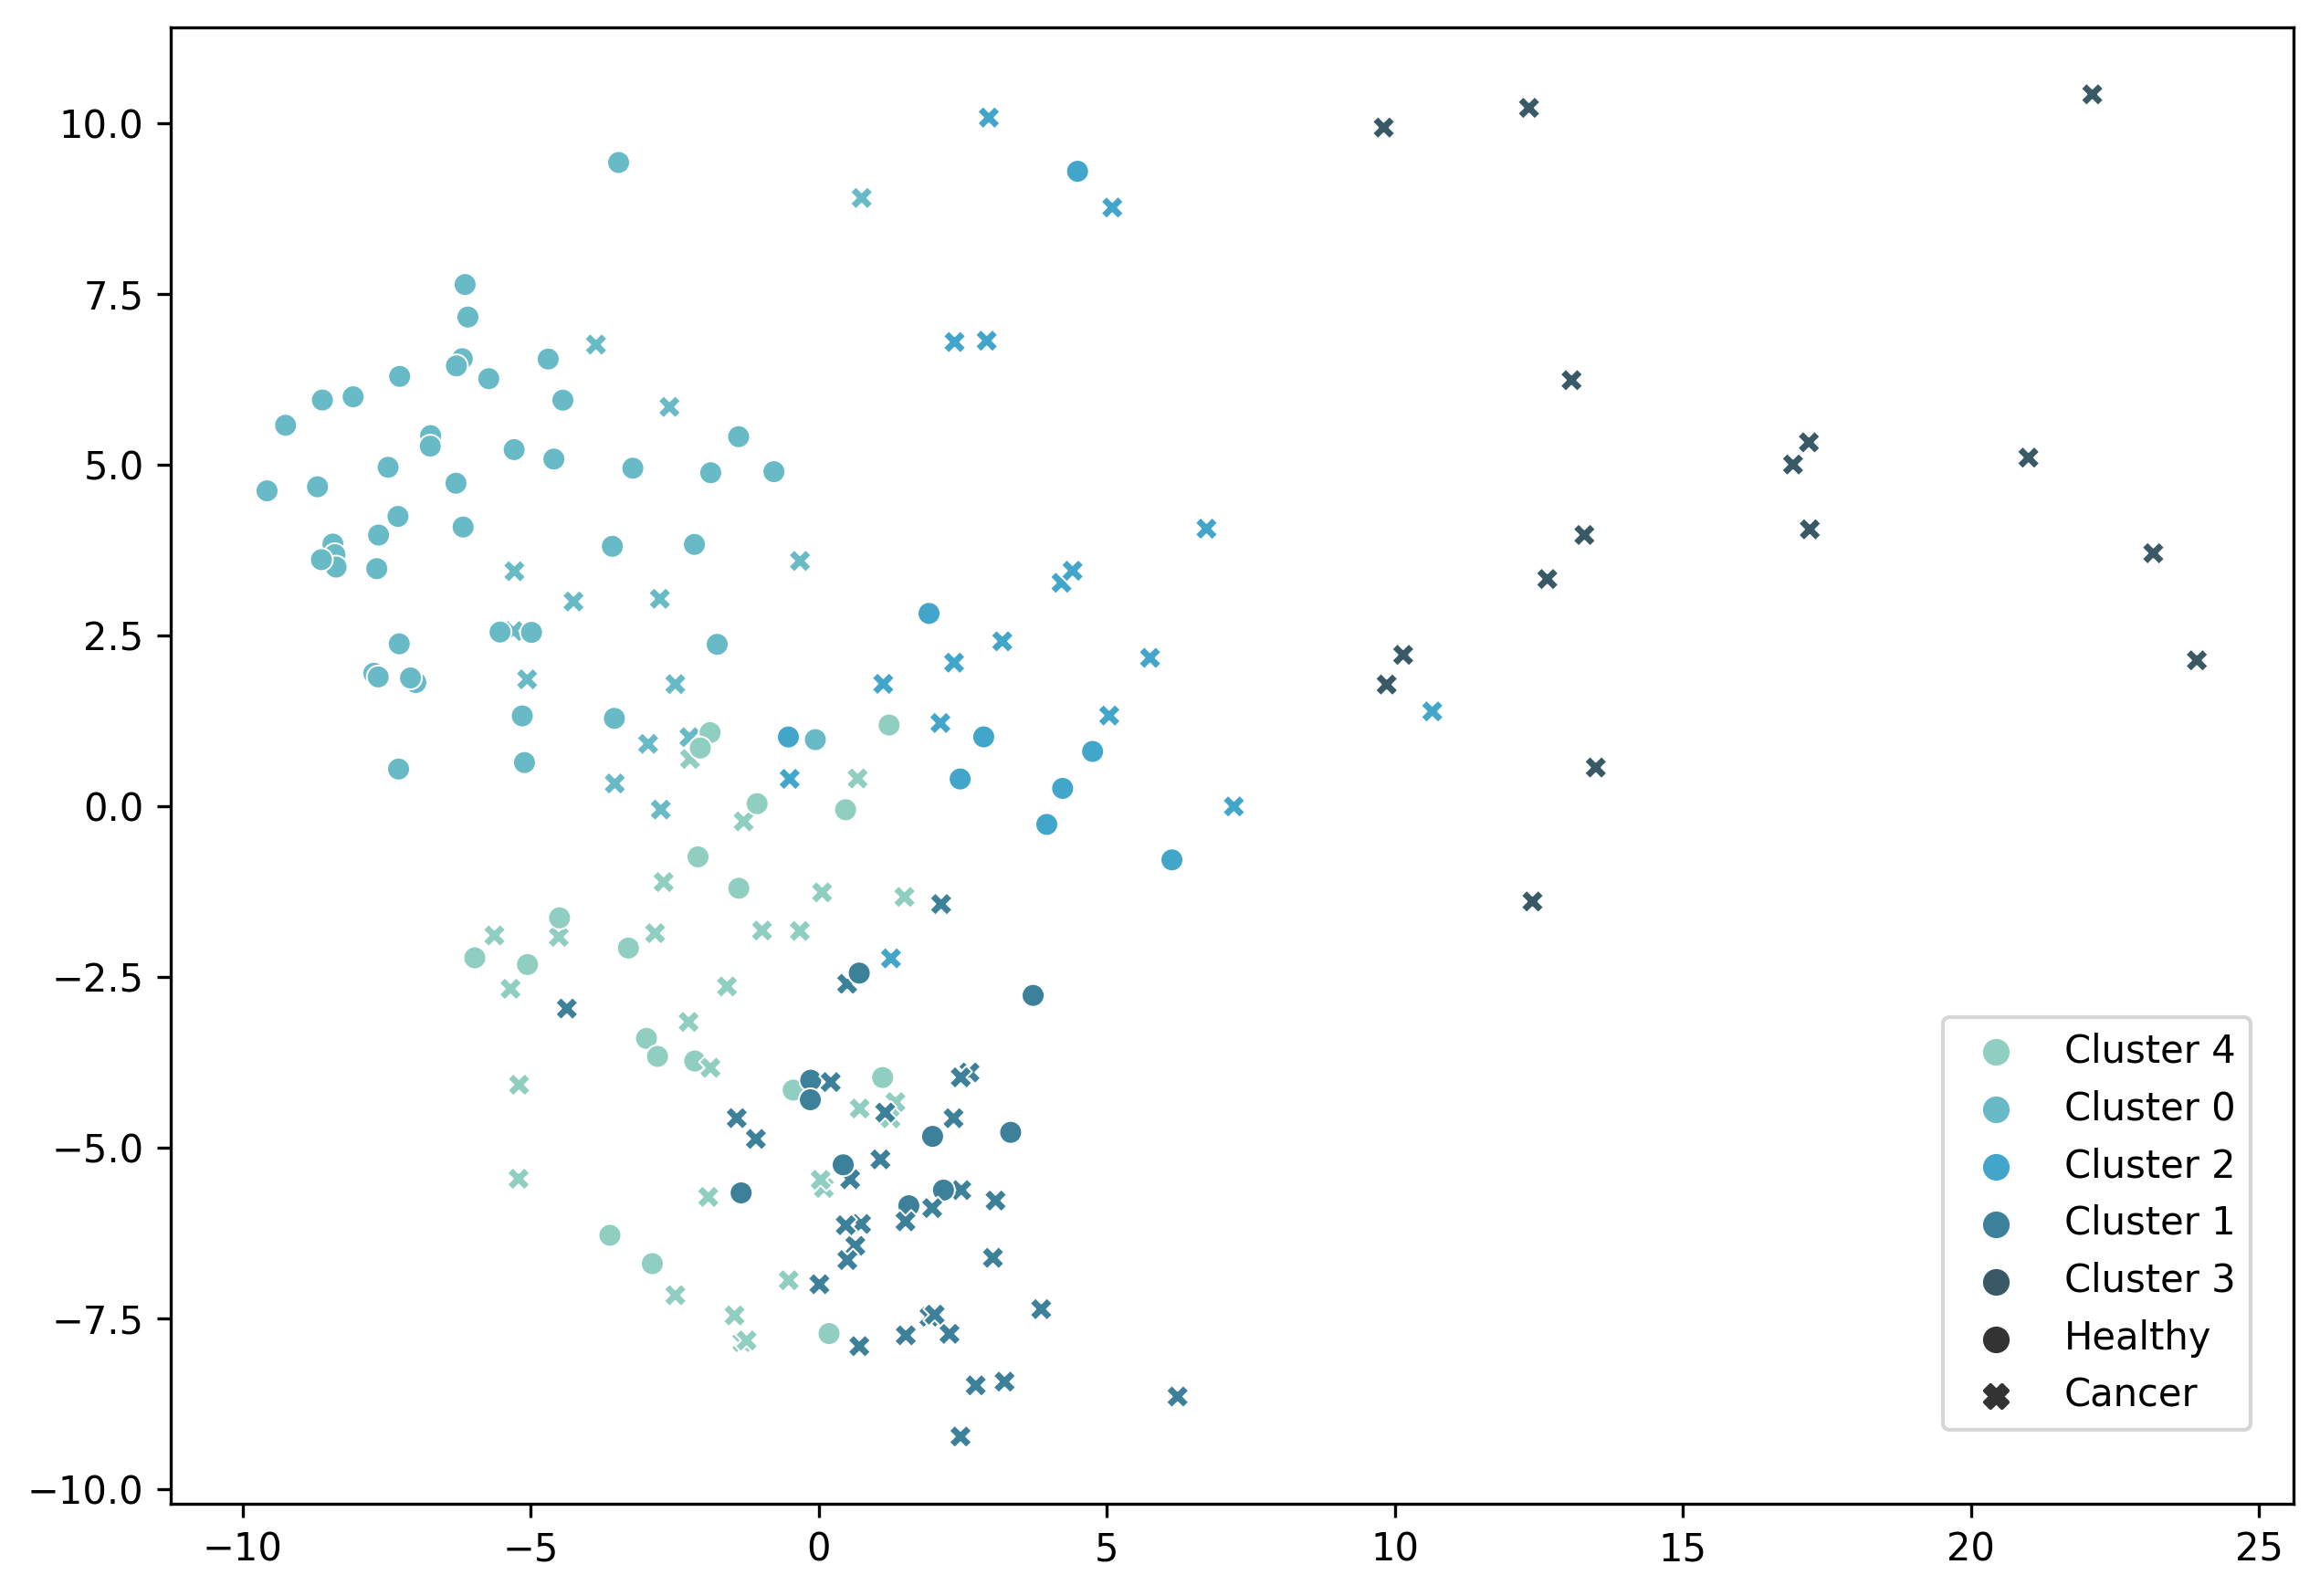
\includegraphics[width=\linewidth]{assets/cluster.png} 
    \captionof{figure}{PCA visualization of K-Means clustering on differentially Expressed genes. Highlighted cancer status, $K=5$.}
    \label{fig:kmeans}
\end{Figure}
Before proceeding in data analysis, we had to find a way to perform dimensionality reduction on high dimension microarray data. This dataset came with 22,215 gene expression levels for each patient, which is way too large for being processed with standard machine learning techniques. The way we managed to identify a relevant and discriminant subset of these genes, was through Differential Expression analysis (DE). 
\noindent
We performed this analysis with the help of the R programming language and the use of the tools \textit{GeoQuery} for data gathering and \textit{Limma} for DE analysis (Version 3.16). They are part of the \textit{Bioconductors} R library. 
After having imported the dataset and filled the missing labels, we log-scaled our gene expression levels and then divided our samples in two categories, 1 for patient diagnosed with cancer and 0 for the ones not diagnosed. 
We then made the contrasts matrix and run the fitting of the Limma model. After the limma linear model was fitted, we performed the empirical bayes statistical test and finally retrieved a list of meaningful genes by invoking the \texttt{topTable} method.
We were finally left with 141 genes ($p=0.01$). Since the dataset uses custom names for genes, we then associated a common name to the biomarkers we just found. We finally exported the obtained data in order to perform further analysis.

\subsection{Unsupervised learning}
After the Differential Expression analysis phase, we decided to run analytics with standard unsupervised machine learning techniques, in order to assess the quality of our biomarkers and see if they reveal to be discriminative towards both classes. We will take advantage of two main python librarires: \textit{Pandas} \cite{reback2020pandas} was used to manage the dataset of gene expression levels and \textit{Scikit-Learn} \cite{scikitlearn} package to perform analytics. 

We started with standard K-Means analysis. after a quick tuning, we found 5 to be the correct number of clusters. This was identified by manually exploiting the elbow method. 
Figure \ref{fig:kmeans} shows the PCA plot of the obtained clusters, and even from this preliminary trial there is a clear distinction among the two classes; in the bottom left of the chart the two classes seems to be overlapped, for this reason we expect to be this a problem for simple classifiers. In addition, as reported in Figure \ref{fig:hist}, cluster 0 contains the larger part of the negative subjects, while cluster 1, 3, and 2 are mainly composed by samples belonging to the positive class. We also decided to run hierarchical clustering. Ward linkage was the best found, and we again were left with five clusters; samples distribution is similar to the one obtained for K-Means. Figure \ref{fig:hcluster} shows the obtained dendrogram. Density based clustering did not provide any significant result on this dataset.

\begin{Figure}
    \centering
    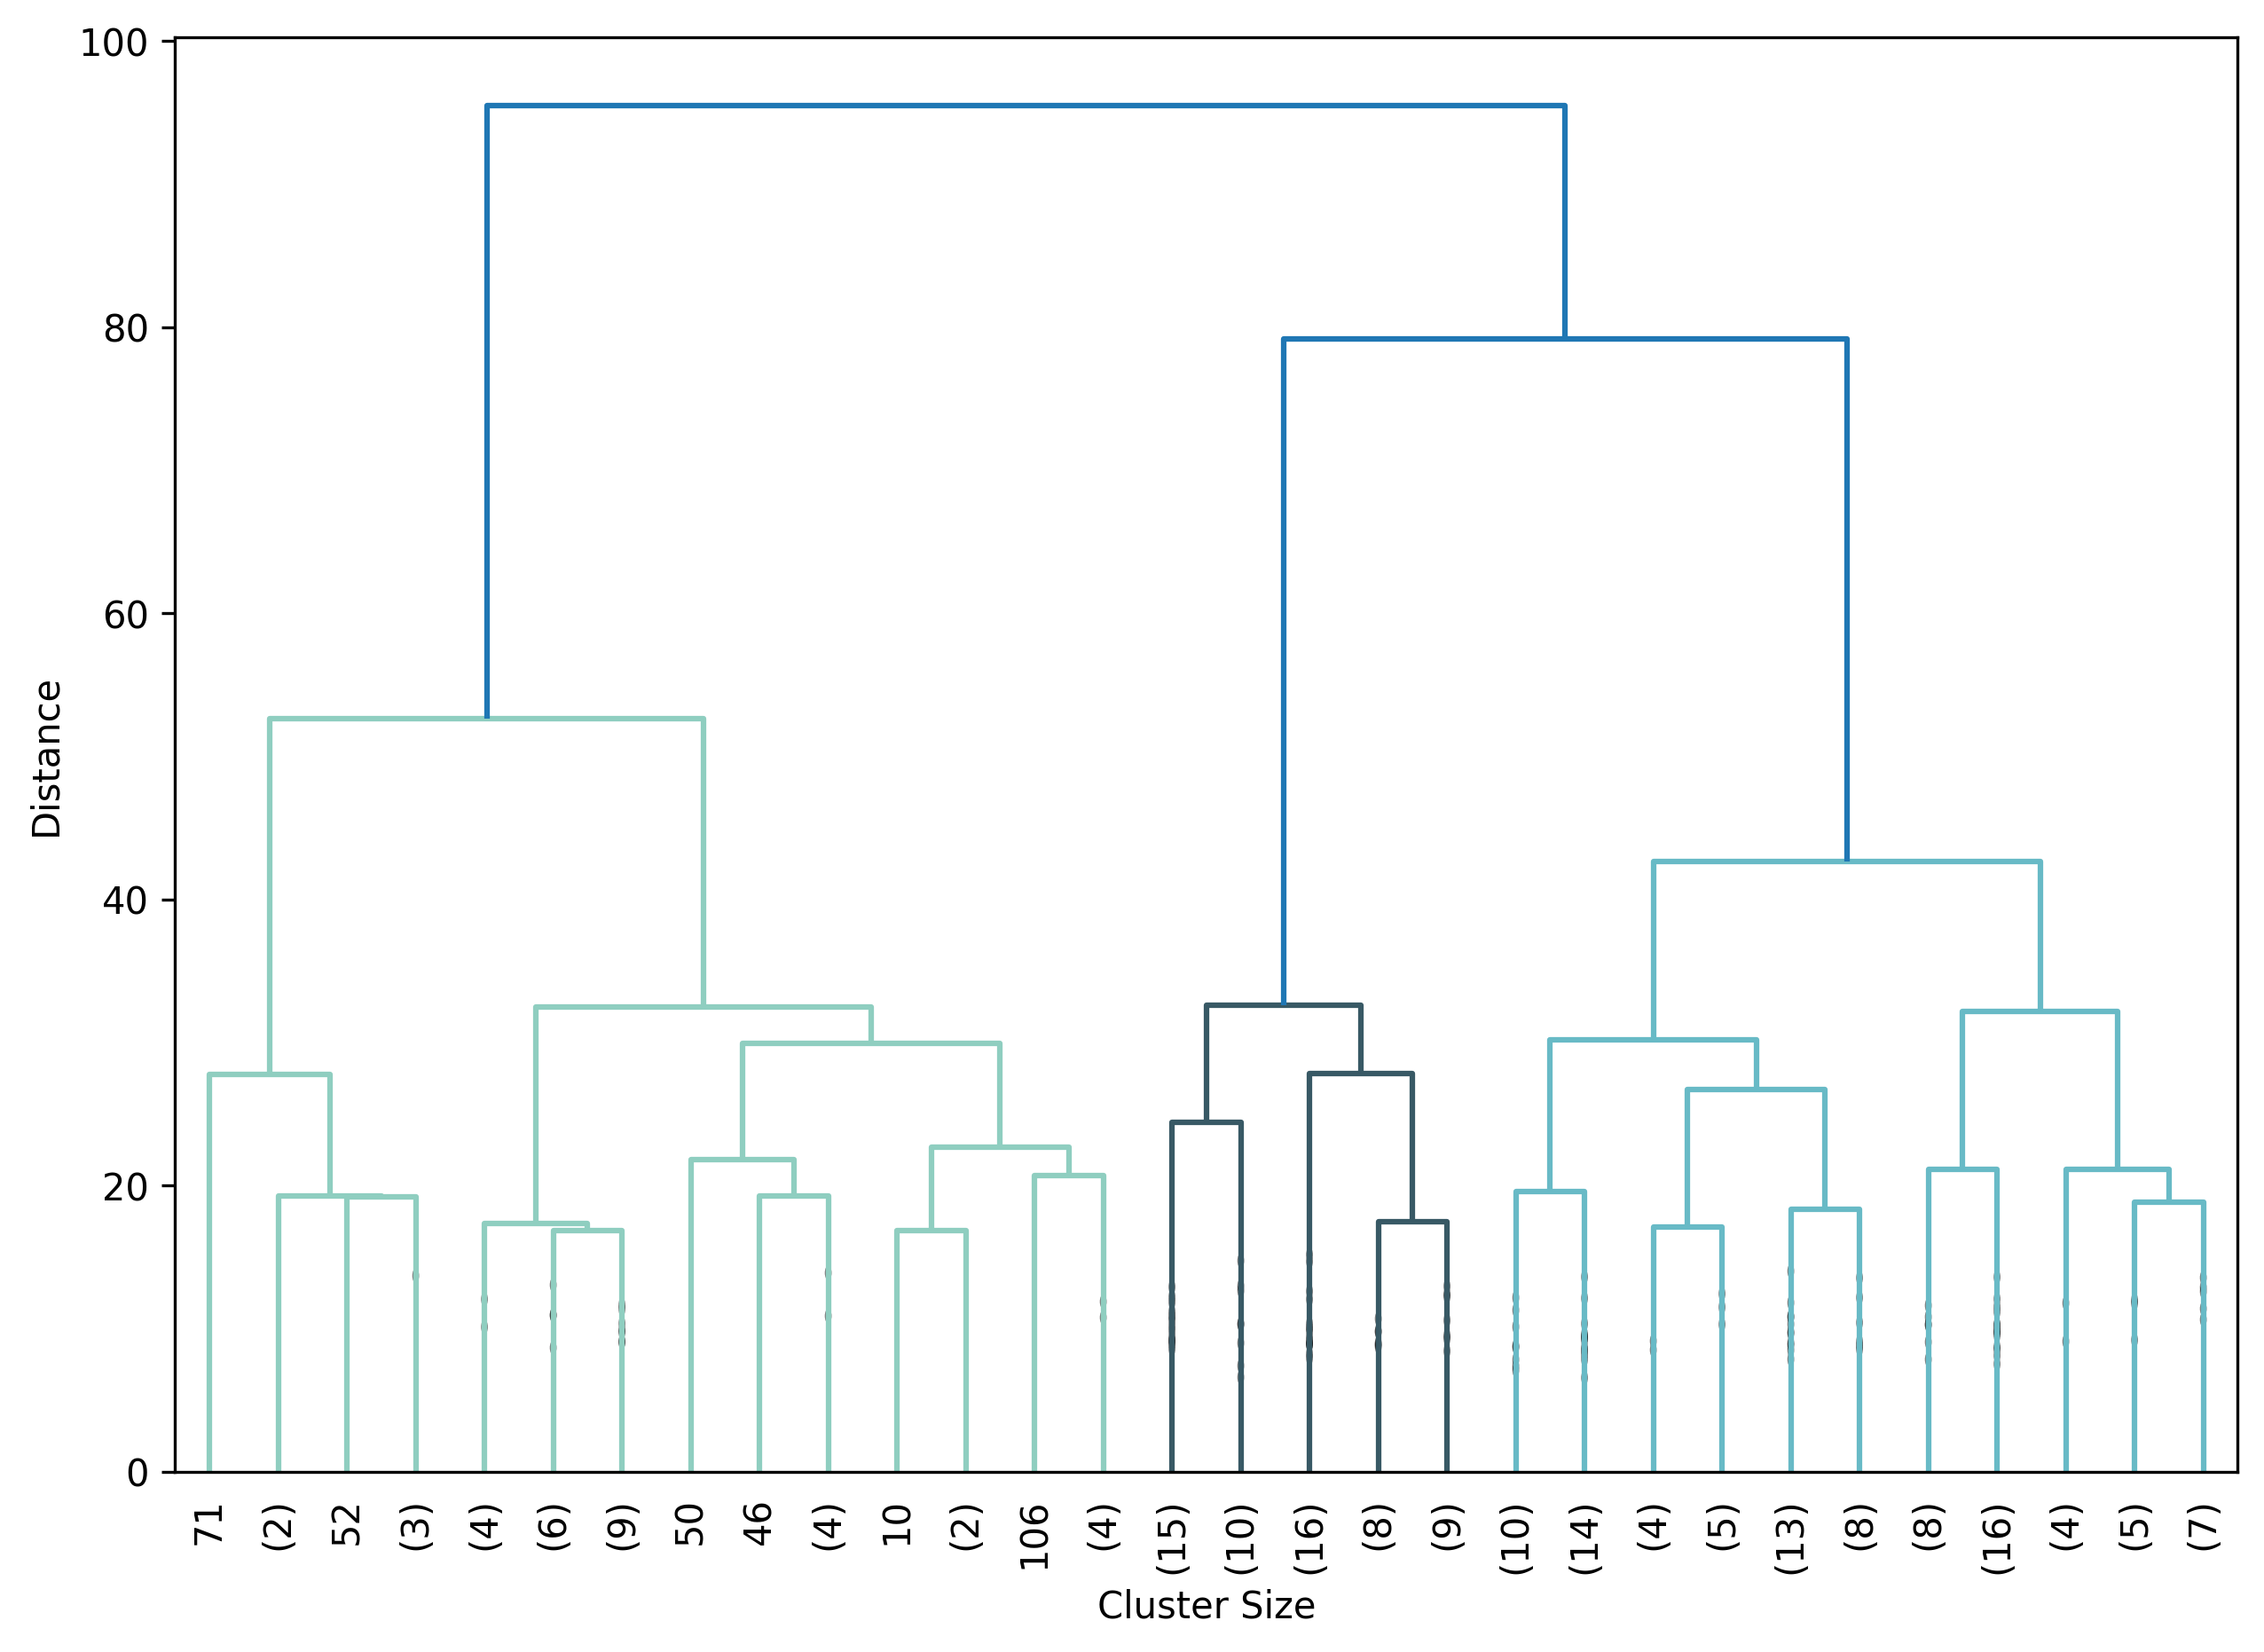
\includegraphics[width=\linewidth]{assets/hcluster.png} 
    \captionof{figure}{Dendrogram obtained after hierarchical clustering. Ward linkage.}
    \label{fig:hcluster}
\end{Figure}

\end{multicols}

\begin{figure*}[!t]
    \centering
    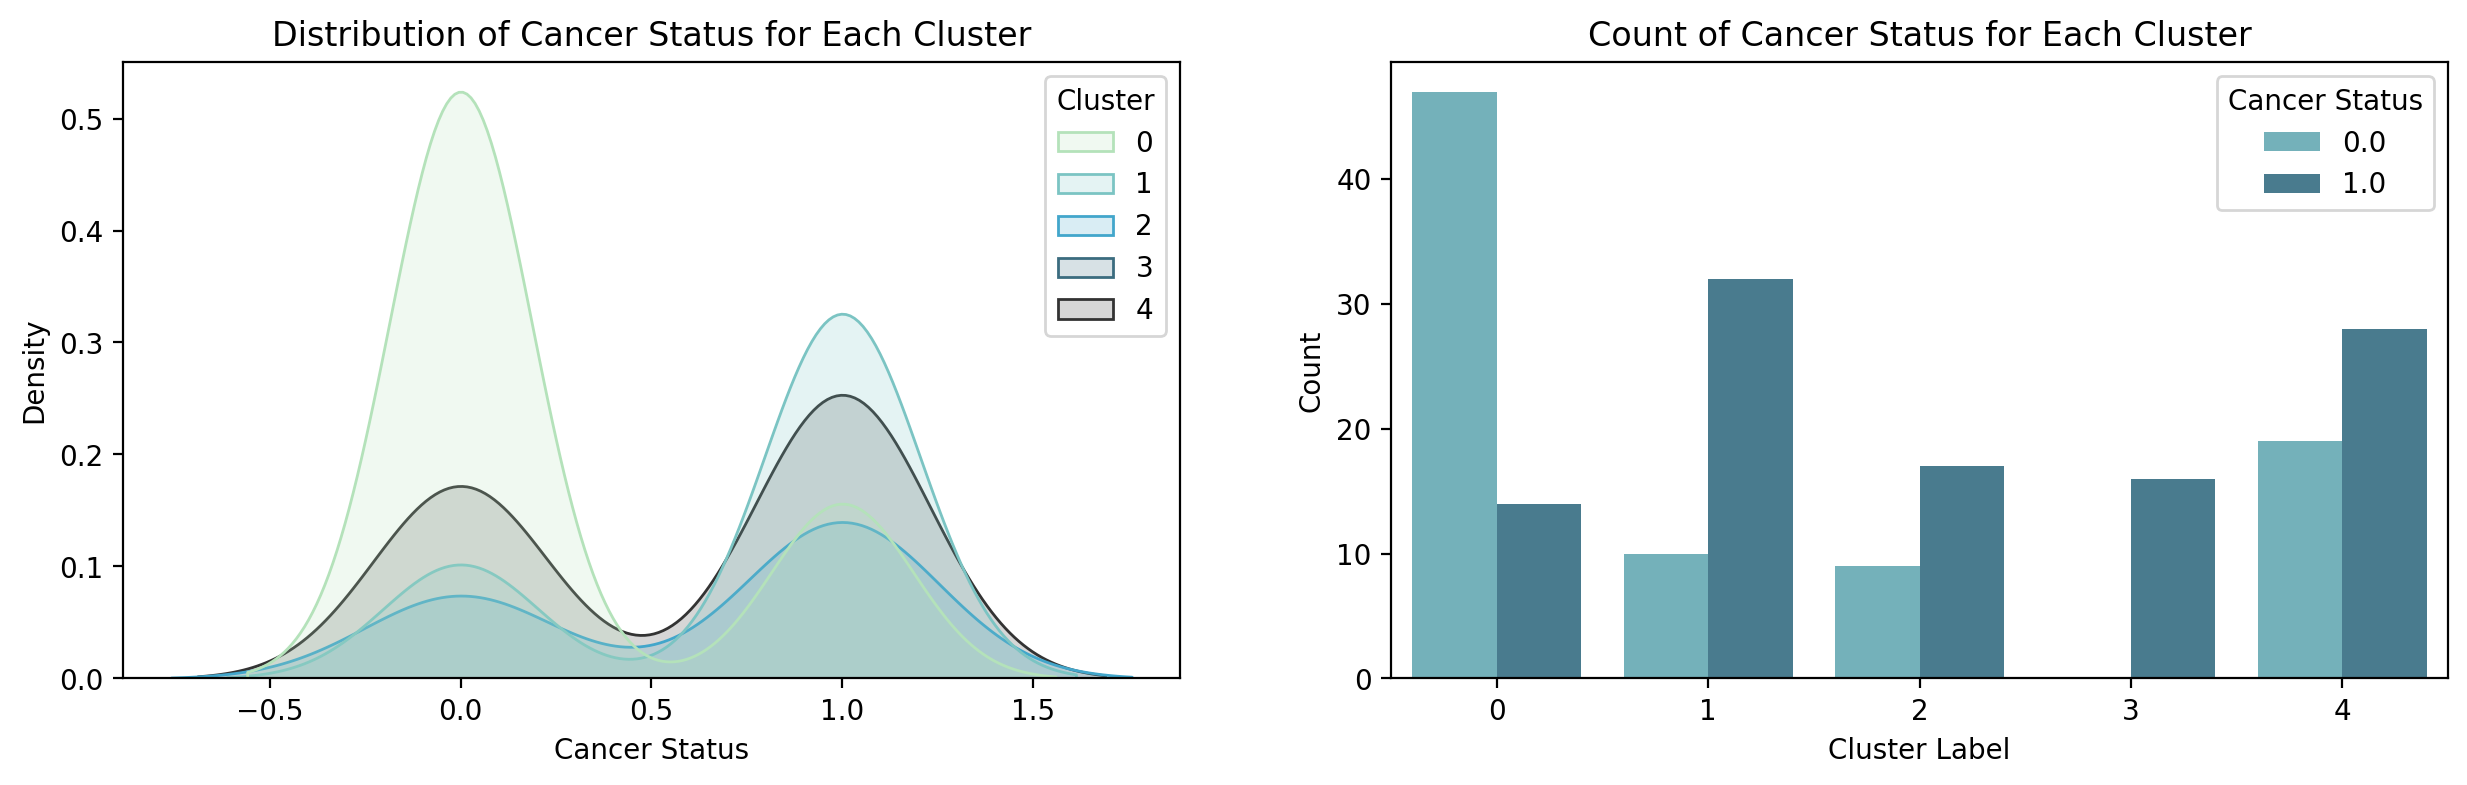
\includegraphics[width=\linewidth]{assets/hist.png} 
    \captionof{figure}{Distribution of cancer status for each cluster.}
    \label{fig:hist}
\end{figure*}
\newpage
\begin{multicols}{2}
[
\section{Classification with Graph Convolutional Neural Networks}
\label{sec:3} 
This section will treat about the main project topic: infer an underlying structure in protein-protein interaction among the previously obtained biomarkers in order to achieve better generalization capabilities in machine learning classification tasks. We will describe in detail how we managed to build a graph to model interactions and we will also provide a gentle mathematical introduction to the machine learning model we used for our scopes. We will finally describe the model validation phase and the obtained results, with an in-depth comparison among different machine learning models. Before proceeding, it is important to mention that all the following analysis was performed using the python programming language by importing the data obtained from the differential expression analysis. All the gene expression levels and numerical features were standardized by removing the mean and scaling to unit variance, and then re-scaled within the (0,1) interval.
]
\subsection{Protein-protein interactions}
Differential expression analysis left us with 141 biomarkers that can discriminate among healthy and ill subjects. Now, we want to find if known relationships among these genes exists, in order to build a graph of the interactions. To achieve this result, we decided to rely on the \textit{BioGrid} database \cite{biogrid}. BioGrid is a public collection of known protein to protein interactions, revealed among different biological species. It comes with a simple REST API that can be queried. With this said, we built a python script on top of the BioGrid REST specification, able to query the database and return for each one of our biomarkers an eventual list of genes the biomarker interacts with. Then, we made the intersection among the returned list and the original biomarkers collection. If the intersection result is not empty, it means that there is an interaction among the queried biomarker and other differentially expressed genes. We then save the intersection and we will use it to build an adjacency matrix, paying attention to remove self loops.
At the end of this process, we obtained a single, structured collection of interactions among our biomarkers: in other words, we managed to build a graph.
%%%%%%%%%%%%%%%%%%%%%%%% ALGORITMO %%%%%%%%%%%%%%%%%%%%%%%%
\begin{algorithm}[H]
\caption{Construct the adjacent matrix}\label{alg:cap}
\begin{algorithmic}
\State biomarkers $ \gets$ list of biomarkers;
\State interactions $ \gets \emptyset$;
\State adj $ \gets zeros(141, 141)$;
\For{$gene \in biomarkers$}
\State response $ \gets $ QueryBiogrid(gene);
\State interactions $ \gets response \cap {biomarkers}$;
\For{$i \in $ interactions}
\State adj(gene, i) $ \gets 1$;
\EndFor
\EndFor
\State \Return adj;
\end{algorithmic}
\end{algorithm}
%%%%%%%%%%%%%%%%%%%%%%%% FINE ALGO %%%%%%%%%%%%%%%%%%%%%%%%
 Algorithm \ref{alg:cap} summarizes the procedure employed.

\noindent
The graph we obtained was finally composed by a connected component of 79 genes and 134 edges. The other genes showed no correlation with the others: we did not remove them, as they are pieces of information as well.
After having asses the graph topology, that is shared across all patients, we filled the nodes with the gene expression levels for each biomarker. At this point we obtained a unique structured representation for each of our samples. Figure \ref{fig:graph} shows the graph that will be exploited in Section \ref{sec:3}. 

\begin{figure*}[!b]
    \centering
    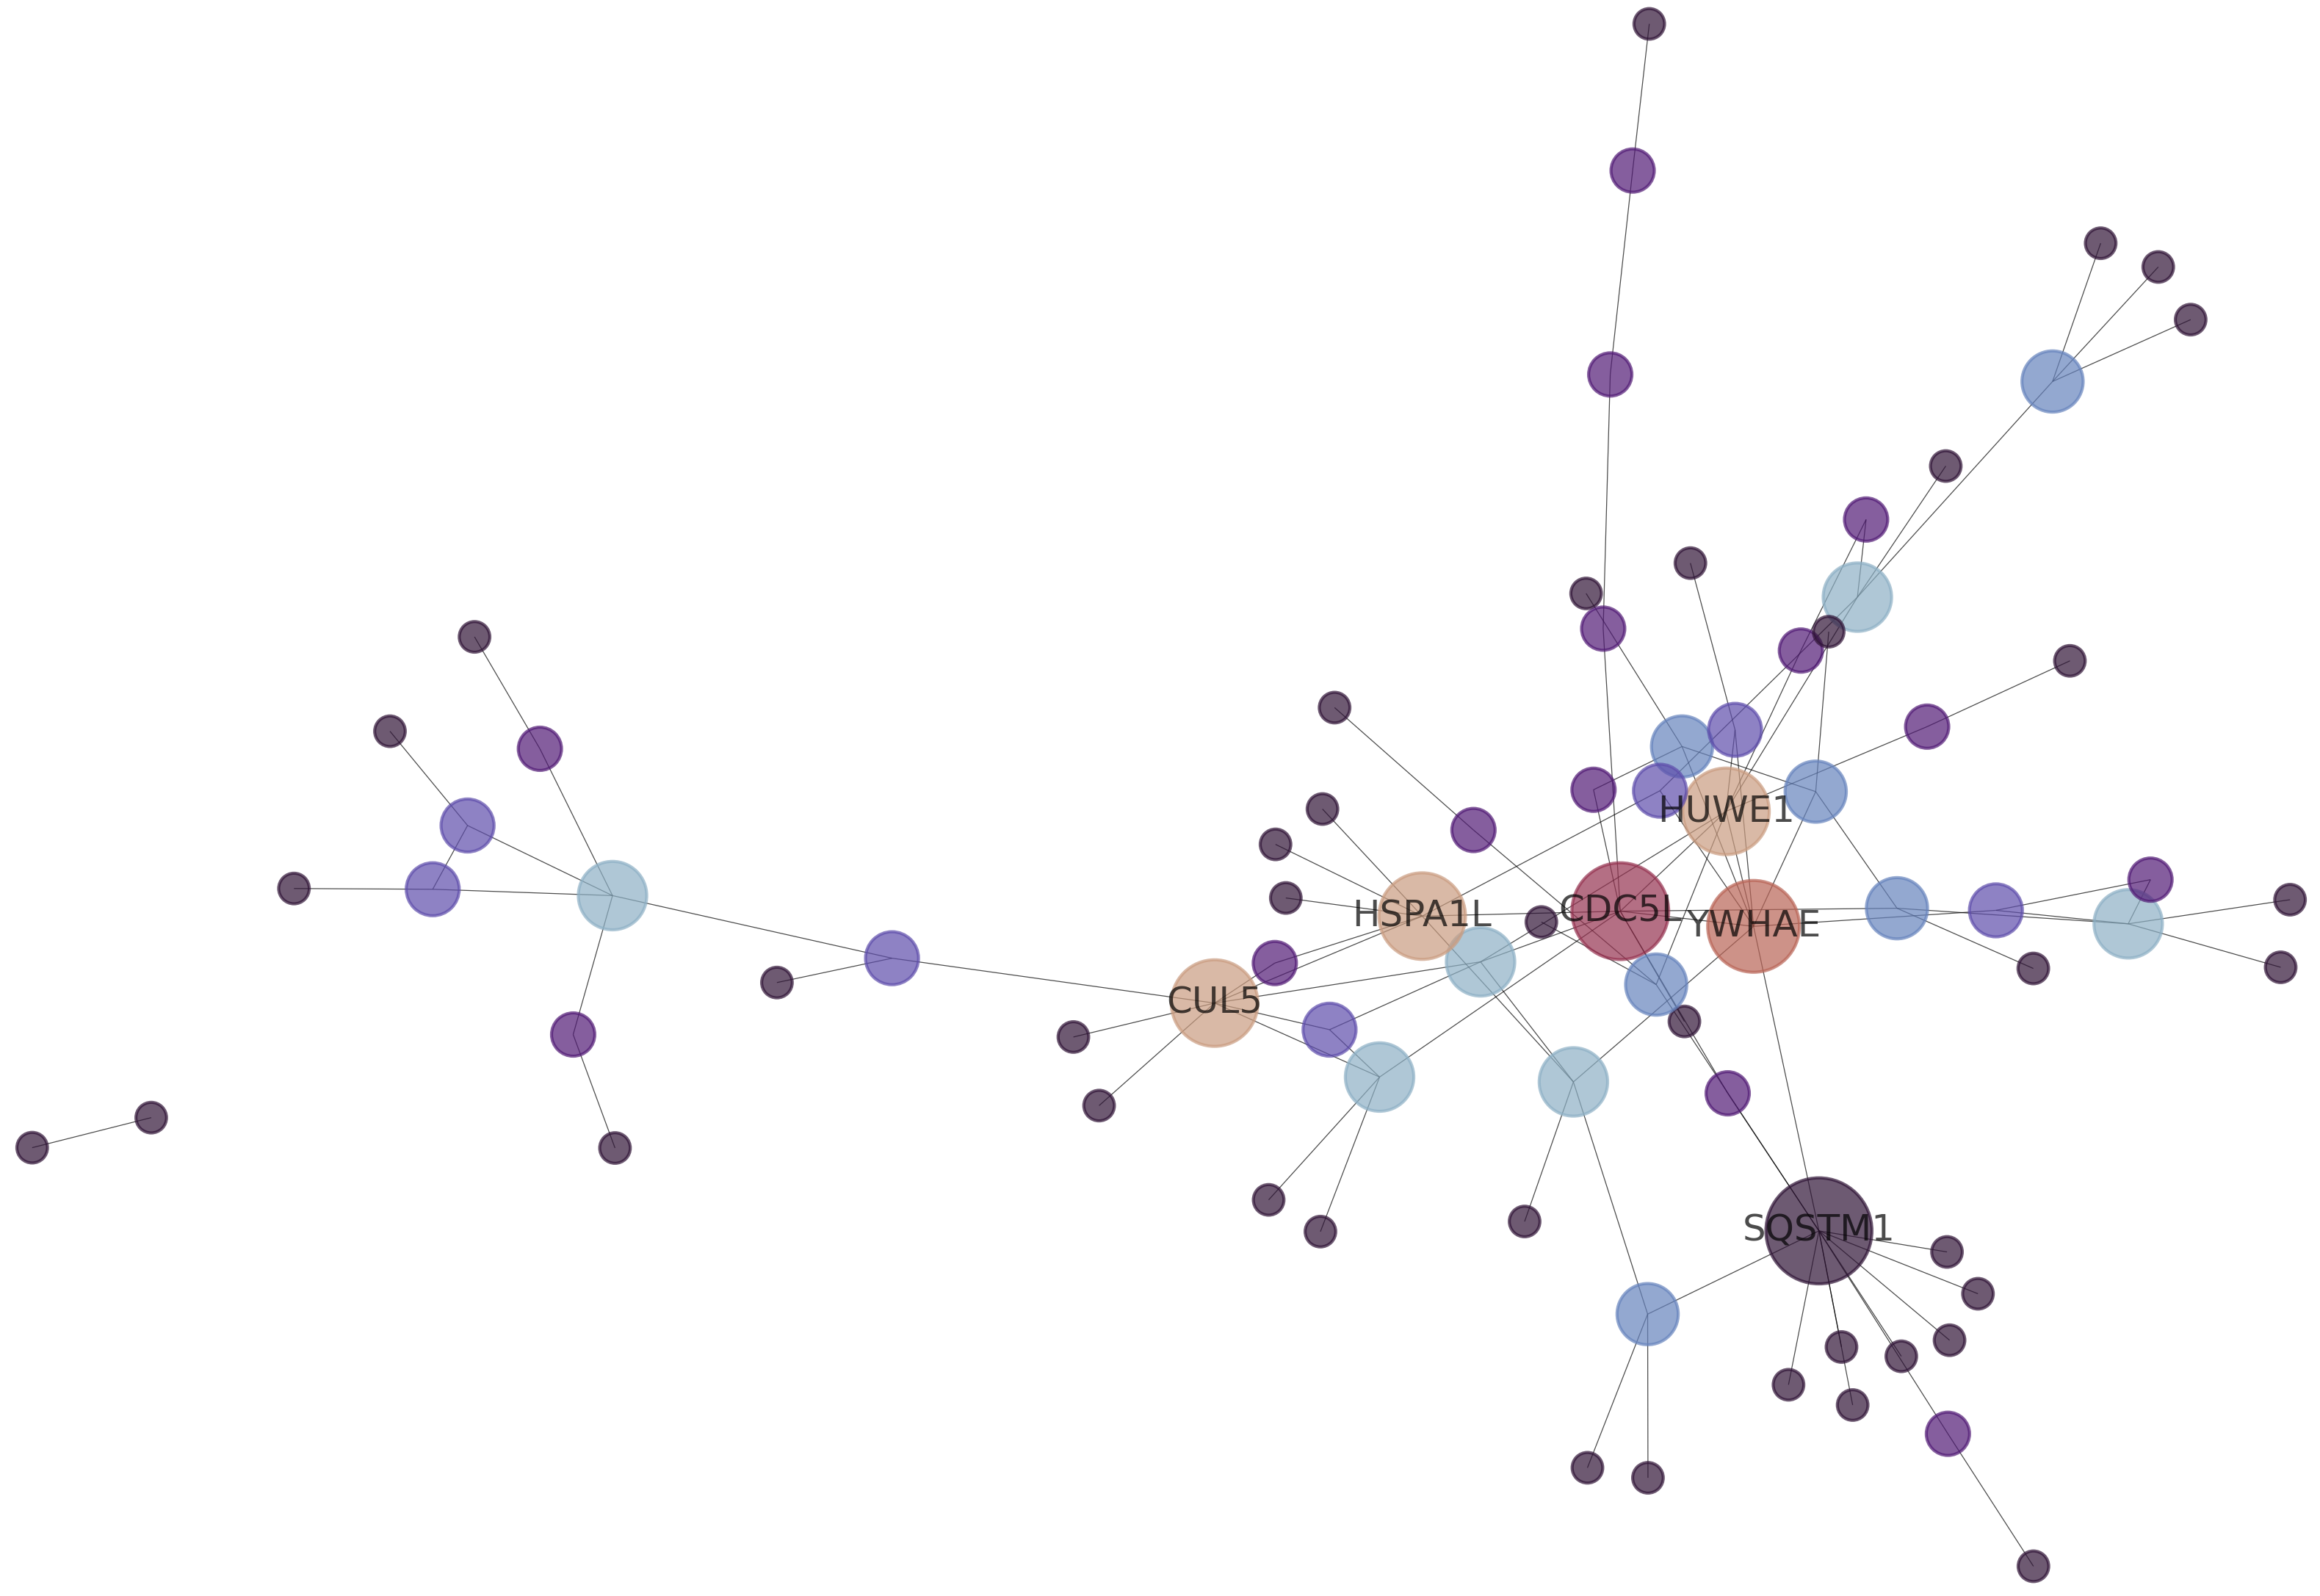
\includegraphics[width=0.6\linewidth]{assets/graph_12345.png} 
    \captionof{figure}{The obtained graph of biomarkers interactions. Node dimension is proportional to its degree; There are six main genes that probably drive the pathway. Singletons nodes were removed for ease of representation}
    \label{fig:graph}
\end{figure*}

\subsection{Introduction to graph neural networks}
Graphs neural networks are a relatively new class of machine learning models that are specifically built for generating an embedding given a graph in input. For this project purposes, we decided to employ a standard Graph Convolutional layer \cite{gcnconv}. More precise formulation of the embedding generated can be found in equation \ref{eq:gcnembedding}

\begin{equation}
X' = \sigma(\hat{D}^{-\frac{1}{2}}\hat{A}\hat{D}^{-\frac{1}{2}}XW^{(l)})
\label{eq:gcnembedding}
\end{equation}
\noindent
being $A$ is the graph adjacency matrix, $\hat{A} = A + I$ the adjacency matrix with self loops inserted, $\hat{D}_{ii} = \sum_{j=0}{\hat{A}_{ij}}$ representing the diagonal degree matrix and $W^{(l)}$ is a set of trainable parameters for a convolutional layer $l$; $X$ is the matrix of features of the graph\footnote{In the general formulation it was supposed to have a tensor of featues for each node. In this case, since we have only one scalar label per node, graph node's matrix will be a vector. } (in other words, it is a matrix containing all graph node's labels). We finally apply non-linearity (ReLU, GeLU \cite{hendrycks2020gaussian}) to the obtained embedding. In conclusion, this layer extends the concept of convolution to graph and message-passing \cite{Bacciu_2020} networks, allowing us to build a simple but effective model trainable by backward propagation. A nice and efficient implementation of this can be found inside the \textit{Pytorch Geometric} \cite{Fey/Lenssen/2019} library. For this reason we opted to use \textit{PyTorch} \cite{NEURIPS2019_9015} for developing the whole model as well as for managing the dataset containing the graph structure.

\subsection{General model architecture}\label{subsec:3.3}
Working with graph convolutional neural network is somewhat similar to working with standard convolutional filters, and general model architecture is really close to a classical image classifier. However, in order to make the model work first, and generalize after, we had to make some assumptions relatively to two fundamental aspects.

First, opposite to image CNNs that stack many layers one over another, GNNs have to be quite \textit{shallow}. In fact, stacking layers lead to a big problem, known in literature as \textit{node smoothing} problem: a message passing network will tend to generate closer and closer embeddings as the number of convolutions increase in depth. For this reason, we chose a single-layer convolution. 

The second problem is somewhat related to gradient propagation and differentiability of our neural network. During the preliminary phase, we noticed that using the standard, non-differentiable ReLU function for non-linearity lead to a poor propagation of the gradients. For this reason, we decided to use a new activation function for our neurons: Gaussian error Linear Unit (GeLU), which is differentiable on all its domain, as well as L2 regularization.

After the convolutional layer, as for image CNNs, we need to reduce embedding dimensionality in order to propagate the embedding to a standard Multi Layer Perceptron: this is delegated to the Global Mean Pooling layer, that takes in input a batch-normalized version of the embedding and returns a compressed version, more suitable for our needs. 
Since we have also categorical features in the dataset, we want to make them available to the classifier. We solved this issue by concatenating the flatten and pooled matrix of embeddings with a vector containing a scaled an normalized version of our categorical features. In particular, we chose 7 of the categorical features mentioned in section \ref{ssec:datasetdesc}, removing the columns relative to subjective assessment and the suspect mass size, which we thought they could act as a proxy for the actual sample label.
\begin{Figure}
    \centering
    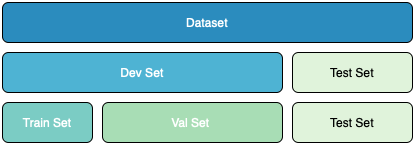
\includegraphics[width=0.9\linewidth]{assets/split-boarder.png} 
    \captionof{figure}{Dataset split.}
    \label{fig:datasplit}
\end{Figure}
Finally, having obtained the final vector of features, we pass it through a GeLU activated MLP which performs the actual classification. Now that we have assessed a draft of our architecture, we can move to the model selection phase that will provide us the right hyperparameters configuration for our task.
Figure \ref{fig:architecture} shows the final chosen architecture for our neural network.

\subsection{Model selection}
In order to assess the perfect hyperparameters configuration for our model, we opted for a standard hold-out validation technique.
We divided our dataset in two splits: a \textbf{developement set} containing 70\% of our data, and a \textbf{test set} with the remaining 30\% portion. Figure \ref{fig:datasplit} graphically shows the performed split. Note that we made sure that class were balanced in every partition of our data split.
\noindent
We will keep the test set for a blind risk assessment procedure after the model selection phase. The actual hyperparameter tuning phase was entirely run by dividing the dev set into another 70/30 split: the first will be used to train the model, and the second will be used to fine tune the parameters, as we will choose the configuration minimizing this split's loss. The hyperparameters we searched on are the following ones:

\begin{itemize}
    \item How many convolutional and dense layers, and their respective number of neurons
    \item The optimizer to be used to minimize the loss function, and its parameters (learning rate ($\eta$), momentum ($\alpha$))
    \item L2 regularization strength ($\lambda$)
\end{itemize}

After the grid search, we were left with the following configuration: Adam as optimizer with a learning rate of 0.02; L2 strength $2\mathrm{e}{-4}$; a single convolutional layer with 256 units and a three-layer MLP with 256 (the actual size of the embedding) + 7 units (needed by the categorical features) for the first hidden layer, 32 for the second and two for the last one, as it's the one providing the classification output. On average, we trained the model for around 200 epochs (we used early stopping to prevent overfitting) and we were able to achieve a MSE loss value of $0.09$ in the training set and $0.11$ in the validation split.

\subsection{Model validation}
When working with machine learning, model validation is the most important part of the work. Before proceeding into an iterative validation phase with the found hyperparameters, we decided to re-train our model on the whole developement set: with more data, we hope to train better the model, as we are getting a lower VC-Bound. In this setting, where we do not have a validation set to establish overfitting, we trained the model until we reached a training loss corresponding to the best validation loss we reached during the model selection phase (in other words, we stopped training when we reached a train loss value of 0.09). After that, we finally test our model on the blind test set we left before, getting an F1-Score of \textbf{93.2}\% in discriminating the positive towards the negative class. 

\begin{Figure}
    \centering
    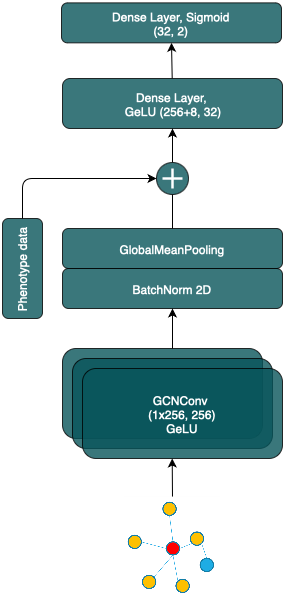
\includegraphics[width=0.8\linewidth]{assets/gnn.drawio-luca.png} 
    \captionof{figure}{Final Model chosen architecture}
    \label{fig:architecture}
\end{Figure}

\noindent
After this hold-out validation, we decided to run a K-Fold cross validation procedure, in order to better assess generalization capabilities of our GNN. We opted for a 3-Fold cross validation, since we used 30\% of our dataset for test during the previous phase. In order to divide the dataset, we again relied on the \textit{scikit-learn} library. We split it three times, each time taking independent folds for training and test set; we then trained the model on the train set, and tested it on the fold's test set. Table \ref{table:results} reports the obtained results in a schematic way.

\begin{center}
\begin{tabular}{ |c|c c|}
\hline
\textbf{Fold} & \textbf{Train F1 (\%)} & \textbf{Test F1 (\%)}\\
\hline
    1 & 91.1 & 93.2 \\
    2 & 92.2 & 81.3 \\
    3 & 90.6 & 85.0 \\
    \hline
    \rowcolor{LightCyan}
    \textbf{Average} & & \textbf{86.7} \\
\hline
\end{tabular}
\captionof{table}{Summary of K-Fold Cross Validation}
\label{table:results}
\end{center}


\subsection{Results}
The selection and validation phase returned us the final model which performance looked really promising in terms of generalization capability. After that, to assess the quality and actual superiority of our solution, we conducted a thorough comparison between our model and other standard classifiers. The results, as depicted in Figure \ref{fig:compare}, unequivocally demonstrate the good performance of our model, surpassing traditional machine learning techniques. A total of four additional model was involved in our comparison: K-Nearest Neighbors (KNN), Random Forest (RF), Support Vector Machine (SVM) and Multi-Layer Perceptron (MLP). In order to produce comparable results, we ran all tests on the same five fold of data. Each model was tested with only the phenotype data, the gene expression values and both data combined together. For the comparative model we basically merge phenotype data with gene expression values in a single input vector. Instead for the Graph Neural Networks model we proceeded to deal with merging structural and categorical features as described in Section \ref{subsec:3.3}.

We used the \textit{scikit-learn} library to define and train the four additional models and, for comparability reason, to ran a coarse grid search for each model. In particular, for the Multi Layer Perceptron (MLP) the hyperparameters searched were the same used for the GNN. Grid search was ran for each of the three input tested.
%Tabella migliori iperparametri???%
Among the evaluated classifiers, K-Nearest Neighbors (KNN) exhibited the weakest performance, as it solely relies on neighboring instances to determine the class of a given node. While Support Vector Machines (SVM) and Random Forest (RF) yielded comparable results when using phenotype data, SVM encountered challenges when confronted with the high dimensionality of gene differential expression values. On the other hand, the Multi Layer Perceptron (MLP) emerged as the sole competitor to Graph Neural Networks (GNNs), achieving an impressive F1 Score of 0.81 when utilizing phenotype data. However, it was the Graph Neural Networks that truly set a significant gap between the previous models, underscoring our solution's remarkable ability to effectively leverage the structural information encoded in the biomarkers.

These findings substantiate the promising potential of integrating structural information into the data, showcasing a significant boost in the performance of our model. Despite these achievements, it is crucial to address some remaining challenges, such as assessing the model's generalization capability on different datasets and exploring its applicability to other diseases. By addressing these areas, we can further solidify the significance and practicality of our approach in the field of machine learning for healthcare.

\end{multicols}

\begin{figure*}[!t]
    \centering
    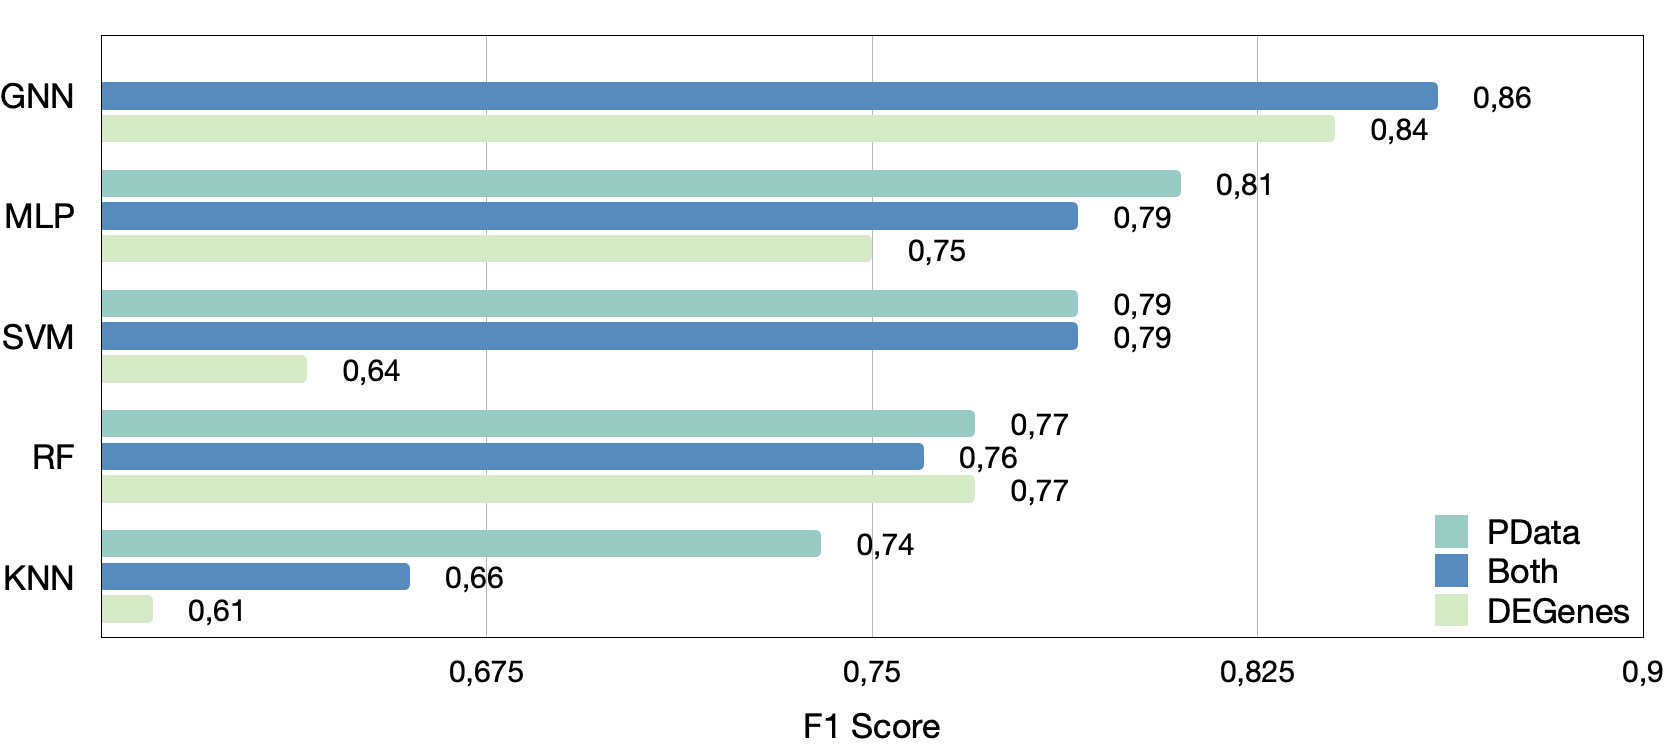
\includegraphics[width=\linewidth]{assets/compare3.png} 
    \captionof{figure}{Comparison of Graph Neural Network F1 Score with respect to other machine learning models.}
    \label{fig:compare}
\end{figure*}


\begin{multicols}{2}
[
\section{Conclusions} \label{sec:4}
]
In this project, we proposed a novel approach for analyzing gene expression data and identifying relevant biological pathways for lung cancer diagnosis. Using a GNN, specifically a graph convolutional layer, we learned the latent features of the graph and performed classification to identify relevant biological pathways for lung cancer diagnosis. Our results demonstrated that our GNN-based approach outperformed traditional machine learning methods in accurately identifying these pathways. The graph convolutional layer allowed us to capture the complex relationships and interactions among the biomarkers, leading to improved classification performance.

The results of our study are promising, as the incorporation of structural information into the data has led to a significant increase in the performance of the model. This finding highlights the importance of considering structural features when analyzing and modeling complex datasets. However, there are still some challenges that need to be addressed in future research.

Firstly, it is crucial to assess the actual generalization capability of the model on other datasets. While our study has demonstrated improved performance on the specific dataset used, it is essential to evaluate how well the model performs on different datasets with varying characteristics. This will provide a better understanding of the model's ability to generalize and its applicability in different contexts.

Additionally, further testing of this approach is needed for other diseases. While our study focused on a specific disease, extending this approach to different medical conditions will help determine its effectiveness across a broader range of healthcare applications. By evaluating the performance of the model on various diseases, we can assess its versatility and potential impact in the field of medical research and diagnosis.

In conclusion, the integration of structural information has shown promising results in enhancing the model's performance. However, the generalization capability on different datasets and the applicability to other diseases remain important challenges that should be addressed in future investigations. These efforts will contribute to the development of more robust and accurate models for a wide range of healthcare applications.

% Mostra bibliografia
\end{multicols}
\newpage
\printbibliography[heading=bibintoc]

\end{document}

